\documentclass[12pt,a4paper]{report}

\usepackage[utf8]{inputenc}
\usepackage[T1]{fontenc}
\usepackage[french]{babel}
\usepackage[margin=0.8in]{geometry}
\usepackage{graphicx}
\usepackage{fancyhdr}
\usepackage[Conny]{fncychap}
\usepackage{setspace}
\usepackage{multirow}
\usepackage{tipa}
\usepackage{textcomp}
\usepackage{amssymb}
\usepackage{lmodern}
\usepackage{soul}
\usepackage{moreverb}
\usepackage{listings}
\usepackage{makeidx}
\usepackage{color}
\usepackage{url}
\usepackage{enumitem}
\usepackage{titlesec}
\usepackage{epigraph}
\usepackage{float}
\usepackage{pdflscape}
\usepackage{tikz}
\usetikzlibrary{arrows,shapes,positioning,shadows,trees}
\tikzset{
  basic/.style  = {draw, text width=4cm, drop shadow, font=\sffamily, rectangle},
  root/.style   = {basic, rounded corners=2pt, thin, align=center,
                   fill=green!30},
  level 2/.style = {basic, rounded corners=6pt, thin,align=center, fill=green!60,
                   text width=8em},
  level 3/.style = {basic, thin, align=left, fill=pink!60, text width=6.5em}
}
\renewcommand{\epigraphsize}{\scriptsize}
\onehalfspacing
\definecolor{rltred}{rgb}{0.85,0.15,0.15}
\definecolor{mil1}{rgb}{0.9,0.1,0.1}
\renewcommand{\footrulewidth}{0.4pt} \renewcommand{\footrulewidth}{0.4pt}
%\DeclareUnicodeCharacter{00A0}{ }
\begin{document}

\begin{titlepage}

\begin{center}
	\begin{tabular}{l l l}
			\begin{minipage}{0.2\textwidth}
			  
\includegraphics[scale=0.3]{ensias.jpg}
			\end{minipage}
			&
			\begin{minipage}{0.46\textwidth}
				\centering
				\scriptsize Université Mohammed V - Rabat \\
				\textcolor{rltred}{E}cole \textcolor{rltred}{N}ationale 
								\textcolor{rltred}{S}upérieure d'\textcolor{rltred}{I}nformatique et 
								d'\textcolor{rltred}{A}nalyse des \textcolor{rltred}{S}ystèmes
			\end{minipage}
			&
			\begin{minipage}{0.24\textwidth}
				\hspace{2cm}
				
\includegraphics[scale=0.4]{logo-ocp.png}
			\end{minipage}
	\end{tabular}
	
	\rule{\linewidth}{1pt}
	
	\vspace{4.65cm}
	
	\huge $Mémoire \ de \ Projet \ de \ Fin \ d\textquotesingleétude$
	
	\vspace{1.5cm} 
	
	\rule{\linewidth}{2pt}
	
	\Large
	\textbf{Analyse de la concurrence du Groupe OCP sur le marché des phosphates et produits dérivés}
	
	\rule{\linewidth}{2pt}
	
	\vspace{1.5cm}
	
	\begin{flushleft}
	
	\normalsize{Soutenu par:} \hfill Membres du jury: \\
	\vspace{10pt}
	\textbf{Hamza SEFIANE \hfill M. Brahim AMRANI (Encadrant interne)} \\
	\textbf{Ayman YACHAOUI \hfill}
	
	\end{flushleft}
	
	\begin{center}
	
			\vspace{72pt}
			\normalsize{Soutenu le x juin 2016} \\
			\vspace{39pt}
			Année Universitaire : 2015-2016
			\vspace{6pt}
			
			\rule{\linewidth}{1pt}
			\footnotesize Av. .Mohammed ben abdellah Regragui, Madinat Al Irfane, Rabat - Maroc\\
			B.P. 713 Agdal - Rabat - Tél. : 05 37 77 73 17 - 05 37 77 85 79 - Fax: 05 37 77 72 30\\
			Site : www.ensias.ma 
	
	\end{center}
	
\end{center}

\end{titlepage}

\chapter*{Remerciements}


\addcontentsline{toc}{chapter}{Résumé}

\chapter*{Résumé}


\textbf{Mots-clés}: 

\addcontentsline{toc}{chapter}{Abstract}

\chapter*{Abstract}



\textbf{Keywords}: 

\tableofcontents
\listoffigures
%\listoftables

\addcontentsline{toc}{chapter}{Introduction}
\chapter*{Introduction}

\epigraph{Economists and agronomists are locked in debate about likely
future yields. Since the method of the economists is to predict
future outcomes from past performance, economists expect
success to continue. And since for the scientists future success
depends on discoveries they will have to make and do not now
know how to make, the scientists are doubtful. At its core, this is
a disagreement about the pace of technical change.}{Robert
Socolow, 1998}
\paragraph{}
Presque toutes les décisions prises par un gestionnaire ont besoin d'une prévision. S'il a une idée de ce qui se passera dans l'avenir, celui-ci peut prendre des décisions de gestion appropriées. Il a également besoin d'évaluer l'effet de ses décisions actuelles sur l'avenir afin que les bonnes décisions soient prises aujourd'hui pour créer une condition souhaitée demain. L’industrie des fertilisants est à forte sollicitation de capital et, par conséquent, sensibles aux variations des coûts. Si nous savons quels types d'engrais sont susceptibles d'être exigés, où et quand, nous pouvons améliorer la qualité des décisions relatives à la production, l'approvisionnement, le placement et la promotion. Par conséquent, nous pouvons minimiser les fonds immobilisés dans les stocks, réduire les coûts d'intérêt, maximiser les réserves en devises étrangères, éviter de manquer de stock et, en général, augmenter les ventes et améliorer les profits.
\paragraph{}
Pour une organisation commercialisant et produisant les engrais, les estimations de la demande et des parts de marché sont indispensables pour les décisions stratégiques et celles concernant l'allocation des ressources. Les pays en développement, confrontés à des problèmes de faible productivité agricole, la croissance démographique et les besoins alimentaires, reconnaissent le rôle crucial des engrais au sein de leur politique de sécurité alimentaire. Les prévisions de la demande d'engrais à court terme et de la consommation potentielle à long terme sont essentielles pour la détermination des politiques appropriées en matière de production alimentaire et l'utilisation des engrais. De même, le mouvement mondial des engrais, leurs tendances des prix et des investissements dans de nouvelles installations de production sont influencés par les attentes de la demande.
\paragraph{}
La puissance de calcul modiale augmentant de façon exponentielle, notre capacité à rassembler, stocker et analyser les données augmente également de façon spectaculaire. Les données sont plus abondantes dans presque toutes les industries et applications académiques. L'industrie agricole ne fait pas l'exception Dans un certain sens, il n'y a plus de données au sein de l'industrie agricole que dans la plupart des autres. L'agriculture est l'un des métiers les plus anciens du monde. Depuis des millénaires, les pratiques agricoles ont été transmises et améliorée. Pendant des siècles, les données agricoles ont été recueillies, suivies et analysées\cite{MIT-BIGDATA}.
\paragraph{}
Les données agricoles sont variées : des rendements des cultures dans certaines zones géographiques aux indicateurs d'érosion, en passant par la météo et les conditions climatiques. Ces données sont collectées, analysées et dans la plupart des cas, partagées par une variété de sources: entreprises privées, des agences gouvernementales et des universités de recherche. Une partie de ces données sont publiées dans des revues, disponibles par le biais des bases de données sur le Web ou vendues par des prestataires d'information. Ces données varient en portée et en exhaustivité; certaines sources de données sont très granulaires tandis que d'autres sont aggrégées.
Les entreprises qui produisent des produits agricoles, les équipes d'ingénieurs R\&D\footnote{Recherche et Développement} et chercheurs recueillent ces données et suivent leurs tendances pour améliorer les semences, les herbicides, les pesticides, les engrais, et la technologie agricole. Les informations et les connaissances acquises par ces entreprises sont généralement brevetées, surveillées, et utilisées à des fins de concurrence dans le marché. 
\paragraph{}
Une fois ces données recueillies, elles sont utilisées par une variété de personnes et d'organisations pour améliorer l'efficacité de l'industrie agricole d'aujourd'hui. Les producteurs individuels utilisent les données des cultures, de la météo et du sol pour prendre des décisions au sujet de leur prochaine saison ainsi que pour pérenniser leurs exploitations. Les entreprises qui fournissent les semences, les produits chimiques, les engrais et d'autres nécessités agricoles surveillent ces données pour créer des prévisions de demande et des plans de production.
\paragraph{} 
Une grande partie de ces données est largement utilisée dans l'industrie. Certains pensent que de meilleures décisions en matière de chaîne d'exploitation et d'approvisionnement pourraient être établies par la compilation minutieuse et l'analyse de segments particuliers de ces données. L'OCP\footnote{Office Chérifien des Phosphates} rejoint ce sentiment.

\chapter{Contexte général du projet}
\epigraph{Economists and agronomists are locked in debate about likely
future yields. Since the method of the economists is to predict
future outcomes from past performance, economists expect
success to continue. And since for the scientists future success
depends on discoveries they will have to make and do not now
know how to make, the scientists are doubtful. At its core, this is
a disagreement about the pace of technical change.}{Robert
Socolow}	
\subparagraph{}
Ce chapitre contextualise le projet dans son environment, en présentant en premier lieu l'organisme hôte de celui-ci – L'Office Chérifien des Phosphates – avant de motiver les raisons inhérentes à son implémentation pour finir sur la planification du déroulement de l'analyse, la conception et la réalisation du projet.
\cleardoublepage

\section{Présentation de l’OCP}
	\subsection{Historique}
	En 1920, alors que partout dans le monde, les compagnies minières fouillent fébrilement le
sous-sol à la recherche du phosphate, minerai aux précieuses vertus fertilisantes, l’Office
Chérifien des Phosphates (OCP S.A. depuis 2008) voit le jour.

En 1965, avec la mise en service du Maroc Chimie à Safi, le groupe devient également
exportateur de produits dérivés. En 1998, il franchit une nouvelle étape en lançant la fabrication
et l’exportation d’acide phosphorique purifié.

Parallèlement, de nombreux partenariats sont développés avec des opérateurs industriels du
secteur, au Maroc et à l’étranger.
	\subsection{Fiche signalétique}
	\begin{description}[align=left]
		\item [Nomination sociale :] Groupe Office Chérifien des Phosphates
		\item [Date de création :] 1920
		\item [Siège social :] 2-4, rue Al Abtal, Hay Erraha, 20200 Casablanca
		\item [Capital social :] 8287 M MAD (2013)
		\item [Effectif employé :] 23,000 (2013)
		\item [Site web :] www.ocpgroup.ma
	\end{description}
	\subsection{Quelques événements marquants de l’histoire du Groupe OCP}
	\begin{description}[align=left]
		\item [1920 :] Création, le 7 août, de l'office chérifien des Phosphates (OCP).
		\item [1959 :] Création de la société marocaine d'études spécialisées et industrielles (SMESI).
		\item [1965 :] Création de la société Maroc Chimie.
		\item [1974 :] Lancement des travaux pour la réalisation du centre minier de Benguérir, en mai.
		\item [1975 :] Création du Groupe OCP avec l'intégration des industries chimiques aux
		\item [1998 :] Le Groupe OCP obtient le Prix National de la Qualité.
		\item [2003 :] L'OCP est devenu le seul actionnaire de Phosboucraâ.
		\item [2008 :] La société anonyme OCP SA est née le 22 janvier - Démarrage de Pakistan Maroc
		\item [2009 :] Démarrage de Bunge Maroc Phosphore à Jorf Lasfar (BMP).
		\item [2010 :] Création de JESA, joint-venture sous forme de partenariat en ingénierie
		\item [2012 :] Creation de la JV BSFT (Black Sea Fertilizer Trading Company)
		\item [2013 :] Signature d’une joint-venture avec Dupont
		\item [2014 :] Inauguration du SLURRY PIPELINE entre Khouribga et Jorf Lasfar
	\end{description}
	
	\subsection{Filiales et Partenariats}
	L'OCP se structure en quatre filières chacune se focalisant sur un segment du groupe OCP et ayant co-créé plusieurs coentreprises dont la figure \ref{fig:mesh1} fait la liste : 
	\begin{figure}[h]
    		\centering
    		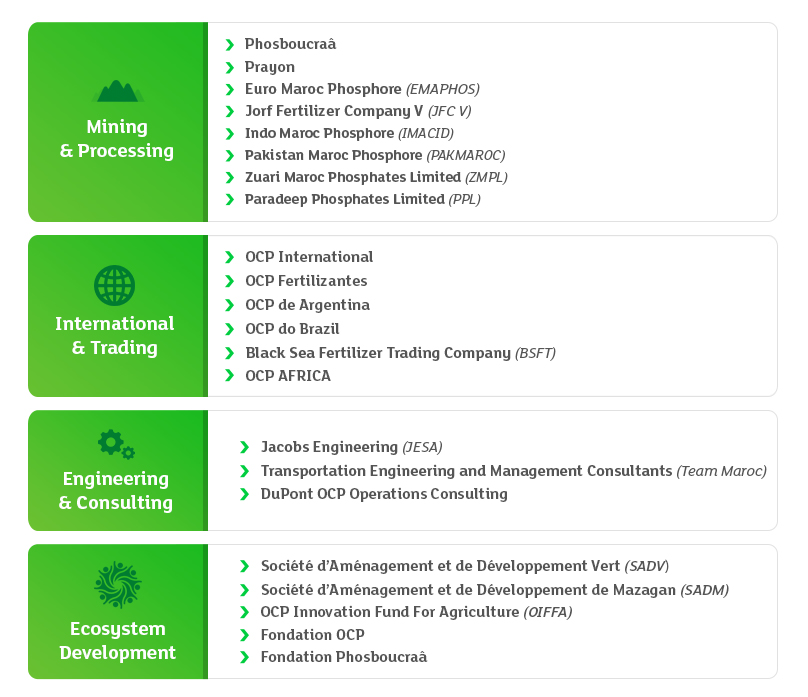
\includegraphics[scale=0.62]{Companies-ocp}
    		\caption{Filiales et Coentreprises de l’OCP\cite{ocp-fil}}
    		\label{fig:mesh1}
	\end{figure}
	
	
\section{Présentation du projet}
	\subsection{Cadre général du projet}
	
	\subsection{Motivation et Problématique}
	\subsubsection{Motivation}
	Parce que la demande d'engrais dépend d'une variété de facteurs agro-économiques, celle-ci n’est pas stable, ni est-elle sujette à des prédictions exactes. Le choix des méthodes de prévision est donc particulièrement important, tant pour la gestion efficiente des compagnies productrices des engrais que pour la formulation de politiques appropriées par les gouvernements.
	La prévision efficace de la demande peut permettre aux exportateurs de tirer pleinement parti des fluctuations des cours mondiaux du marché. Le stockage requis, le transport, les ressources humaines à mobiliser, les arrangements financiers de crédits et de devises étrangères sont tributaires de la demande.
	\paragraph{}
	Considérant que les engrais produits mais non vendus peuvent être conservés pendant un an avant de trouver un acheteur et qu'une durée de stockage d'une année peut causer des partes en quantité et en qualité conséquentes, l'importance de la prévision de la demande peut être facilement appréciée. Si la demande réelle est plus grande que prévue, ce ci conduit à des pénuries, une production agricole inférieure et, souvent, à des implications politiques pour les pays importateurs.
	\paragraph*{}
	Tous les plans des entreprises fabriquant ou commercialisant des engrais devraient être dérivés directement ou indirectement de la prévision de la demande. A partir d'une prévision internationale de la demande, les ventes attendues d'une entreprise peuvent être estimées en évaluant sa part de marché dans chaque région du pays.
	\paragraph{}
	La prévision des ventes servira de consigne à l’égard du département de production quant à quoi, quand et combien produire. Le département financier de l'OCP, lui, est ainsi en mesure de préparer, sur la base des prévisions de ventes, un plan d'entrées et sorties de fonds, évaluer l'écart entre les fonds de roulement et d'organiser le soutien nécessaire de la banque. Le département marketing est guidé par la prévision dans le déploiement du personnel de vente, alors que le logistique sera éclairé quant à l’organisation du stockage à des endroits appropriés, les contrats de transport de marchandises pour faire face au volume prévu de l'entreprise.
	\subsubsection{Problématique}
Au fil des années, la direction commerciale-marketing où nous avons effectué notre stage de fin d'études, a itérativement modernisé ses outils de traitement d'information. Dernière contribution en date de L'ENSIAS\footnote{Ecole Nationale Supérieure d'Informatique et d'Analyse des Systèmes - Grande Ecole d'Ingénieurs, Maroc} à cet essort informationnel, a consisté en la mise en place d'une solution adéquate basée sur les concepts et technologies du BI\footnote{Business Intelligence} ayant permis l'automatisation de la reception, de la normatlisation et l'exploitation de tableau de bord post-analyse des données recuillies\cite{NACER}. La plateforme ainsi réalisée par notre prédecesseur est ainsi un socle pour aider les décionnaires CM\footnote{Commercial-Marketing} à mieux appréhender les évolution et historiques des marchés mondiaux.\paragraph{}Ces données proviennent des organismes indépendants spécialisés dans l'analyse de marché. Hebdomadairement, la direction commerciale reçoit plus de 100 publications de ces organismes qui contiennent des guides de prix, des évaluations ou même des prévisions concernant le marché de phosphates, ses dérivées et les matières premières.\paragraph{}Nous proposons d'emmener les perspectives informationelles du département CM au-delà du reporting \footnote{Tableaux de bord et rapports Business Intelligence} continu vers des mécanismes décisionnels et prévisionnels mettant en œuvre les techniques à l'état de l'art de fouilles de données (cf def data mining) . Nous souhaitons ainsi 'miner' des relations interessantes régissant le marché international des phosphates qui ne sauraient être mises en relief par les techniques de la BI à savoir la segmentation en faits, dimensions et mesures. Notre problématique s'articule ainsi:\subparagraph*{}\textbf{Quelles mécanismes prévisionnels peuvent être établis à la suite d'une recherche de structure précedemment inconnue dans le marché international des phosphates ?}\subparagraph*{}Répondre d'une manière exhaustive à cette question constituerait un atout clé en faveur d'une meilleure compétitivité de l'OCP et nous nous proposons d'explorer divers piste dont le présent rapport témoigne. 
\section{Planification du projet}
	\subsection{Les étapes CRISP-DM d'un projet Data Mining}
	\subsection{Le planning du projet}

\chapter{Analyse et spécification}
\epigraph{If a student takes the whole series of my folklore courses including the graduate seminars, he or she should learn something about fieldwork, something about bibliography, something about how to carry out library research, and something about how to publish that research.}{Alan Dundes}

\cleardoublepage

\section{Analyse de l’existant}
\section{Revue de littérature}
\subsection{Qu'est ce que le Data Mining ?}
La fouille de données, français pour le "Data Mining" est le processus de recherche et de découverte d'auparavant inconnus et potentiellement intéressants modèles dans les grands ensembles de données \cite{def-DM}. L'information 'minée' est typiquement représentée par un modèle de la structure sémantique de l'ensemble de données, où le modèle peut être utilisé sur de nouvelles données à des fins de prédiction ou de classification. Alternativement, des experts humains du métier en question peuvent choisir d'examiner manuellement le modèle, à la recherche d'éléments qui expliqueraient des caractéristiques précédemment mal comprises ou inconnues du domaine d'étude.
\paragraph{}
Brynjolfsson, Hitt, et Kim\cite{data-driven-des} ont mené des recherches empiriques et ont conclu que la performance des organisations est directement liée à leur capacité à prendre des décisions dirigées par les données. Il est donc important de comprendre les facteurs de succès nécessaires pour adopter des techniques de fouilles de données dans les organisations.
\subsection{Les études de prévisions en matière de fertilisants}\label{read1}
\subsection{Prévision à court-terme de la demande de fertilisants}\label{read2}
\section{Compréhension du problème}
\section{Spécification}
	\subsection{Spécification fonctionelle}
	\subsection{Spécification technique}
	\subsubsection{Outils de réalisation}
		\begin{itemize}
			\item
			\textbf{Python : } 
				\begin{itemize}
					\item[$\textasteriskcentered$] Python est un langage de programmation objet, multi-paradigme et multiplate-forme. Il favorise la programmation impérative structurée, fonctionnelle et orientée objet.
					\item[$\textasteriskcentered$] Il est conçu pour optimiser la productivité des programmeurs en offrant des outils de haut niveau et une syntaxe simple à utiliser.
					\newpage
					\item[$\textasteriskcentered$] \textbf{Pourquoi Python dans notre projet ?}
					\begin{itemize}
						\item[\textbf{+}] Calculatrice vectorielle évoluée.
						\item[\textbf{+}] Traitement de fichier texte.
						\item[\textbf{+}] Scripts, ou commandes Unix pour traitements de fichiers par lots.
						\item[\textbf{+}] Langage "Glue" pour enchaîner les traitements par différents programmes. Exemple : Parsing PDF et enregistrement sur fichiers, repris par un code pour structuration des données et traitement.
					\end{itemize}
				\end{itemize}
			\item
			\textbf{Langage R : } 
				\begin{itemize}
					\item[$\textasteriskcentered$] R est un environnement permettant de faire des analyses statistiques et de produire des graphiques évolués.
					\item[$\textasteriskcentered$] C’est également un langage de programmation complet et mature.Sa licence est open-source, son utilisation est gratuite, même dans le contexte de l’entreprise ou de la formation.
					\item[$\textasteriskcentered$] L’environnement R intégre de nombreuses fonctionnalité pour la manipulation de données, et d’affichages graphiques.
				\end{itemize}
		\end{itemize}

\chapter{Collecte, compréhension et préparation des données.}
\epigraph{“Data! Data! Data!” he cried impatiently. “I can’t make bricks without clay.”}{Sherlock Holmes}
\subparagraph{}
Ce chapitre présente le processus d'acquisition des données et leur préparation pour les besoins d'analyse et de modélisation. Nous décrivons en premier lieu le paysage des données au moment du début de notre stage pour ensuite présenter les opération de consolidation, d'audit et d'extension que nous lui faisons subir.
\cleardoublepage
\newcommand{\reels}{\mathbb{R}}
	\section{Compréhension et préparation des données locales\protect\footnote{Données disponibles au sein du portail Business Intelligence de l'OCP}}
	\subsection{Compréhension des données locales}
	Comme rappelé dans la section \ref{CGP}. Les travaux de nos prédécesseurs dans leurs efforts de moderniser le portail \textit{Business Intelligence} de l'OCP se sont arrêtés à automatiser l'archivage des données se rapportant aux historiques de ventes en terme de prix et volumes en un premier lieu\cite{CHEMLAL} avant de concevoir le socle OLAP\footnote{le traitement analytique en ligne (OnLine Analytical Processing, OLAP)\nomenclature{\textbf{OLAP : }}{OnLine Analytical Processing} est un type d'application informatique orienté vers l'analyse sur-le-champ d'informations selon plusieurs axes, dans le but d'obtenir des rapports de synthèse} dans la vue de générer des rapports synthétiques concernant les historiques des échanges du marché des phosphates ensuite\cite{NACER}.\\
	Seules sont ainsi présentes les données concernant les échanges internationaux en terme de produits phosphatés et ceux-ci sont présents sous deux différentes formes de données.
					\begin{wrapfigure}[9]{r}{5 cm}
						\raggedleft
						\fbox{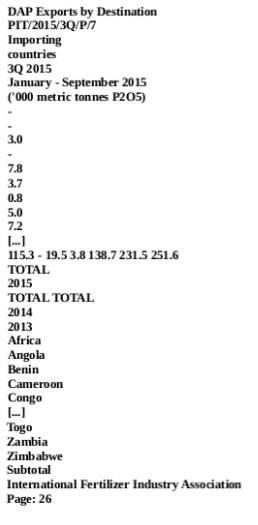
\includegraphics[scale=0.5]{IFA-txt}}
						\raggedleft
						\caption{Lecture "machine" du .pdf de la "Trade Matrix" de la figure \ref{fig:IFA-PDF}}
						\label{fig:IFA-TXT}
					\end{wrapfigure}
	La première est notre format de fichier source: des fichiers .pdf  non structurés vis-à-vis de notre besoin (figure \ref{fig:IFA-PDF}), et qui présentent:
		\begin{itemize}
		\item L'avantage d’être à jour, exhaustifs et dont la véracité est certifiée par un organisme international (IFA\nomenclature{\textbf{IFA : }}{International Fertilizer industry Association})
		\item L’inconvénient d’être flexible pour la lecture humaine mais ne présentant pas une grammaire machine formelle rendant possible une analyse syntaxique, comme en témoigne la figure \ref{fig:IFA-TXT}.
			\begin{figure}[H]
			    		\raggedright
		    			\fbox{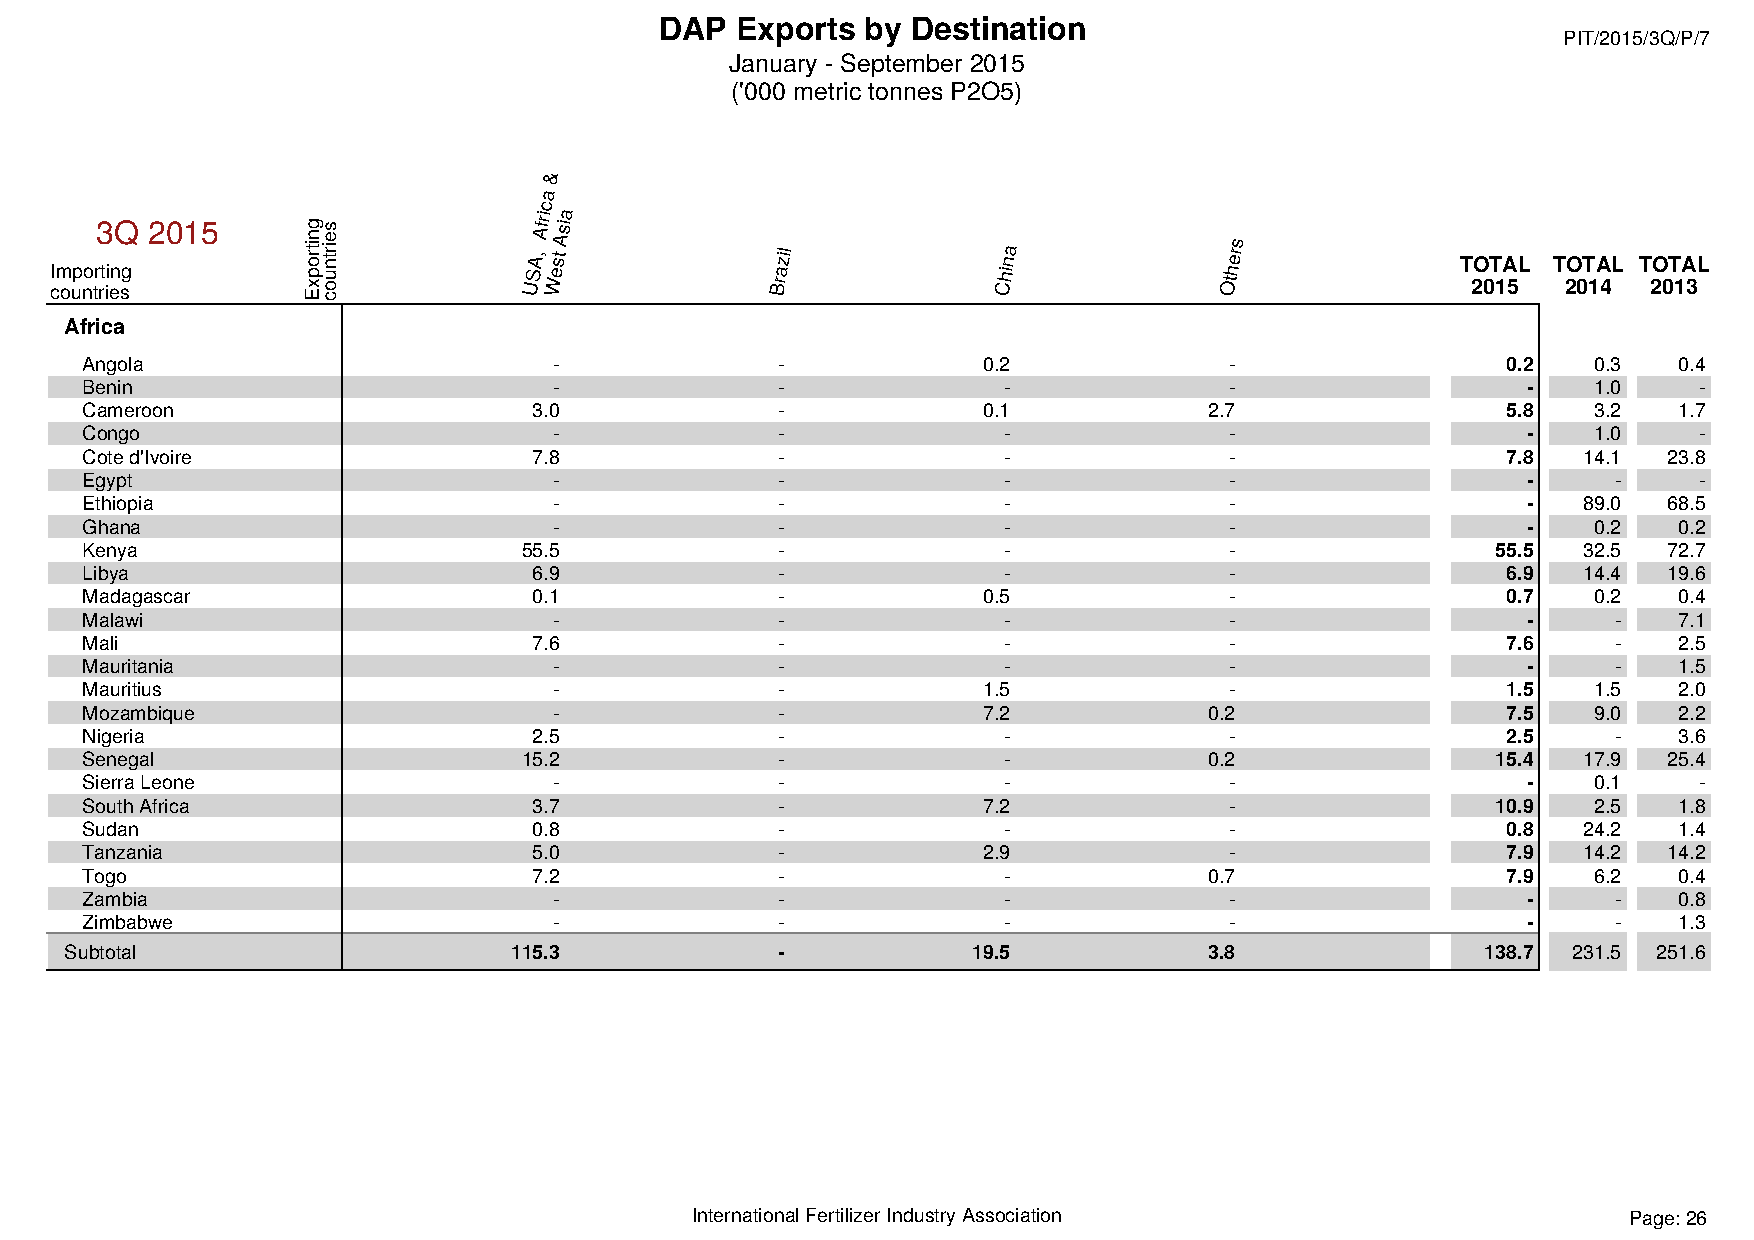
\includegraphics[scale=0.3]{IFA_EX}}
		    			\captionsetup{justification=raggedright,
		    			singlelinecheck=false
		    			}
			    		\caption{Exemple d'une "Trade Matrix"\protect\footnote{Matrice des imports/exports entre les pays du monde, deux-à-deux, des phosphates et produits dérivés} dans le rapport\\trimestriel de l'IFA}
			    		\label{fig:IFA-PDF}
			\end{figure}	
		\end{itemize}
		
		\paragraph{}
		La seconde est structurée dans des datamarts dont une sortie de requête est présentée dans la figure \ref{fig:DMOCP}.
	Ceci est notre format de données cible 
	et présente:
	\begin{itemize}
	\item L'avantage d’offrir le maximum de flexibilité pour le requêtage, et d'être de grande qualité en terme de disponibilité et de véracité, puisque celui-ci a été soigneusement introduit à la main\footnote{À travers une lecture "humaine" des .pdf présentés par la figure \ref{fig:IFA-PDF}}.
	\item L’inconvénient d'être prohibitif en temps et en ressources humaines.
	 En effet, nous avons constaté un retard datant de fin décembre 2013 par rapport aux derniers .pdf reçus par l'OCP.
	\end{itemize}
	\begin{figure}[H]
		    		\centering
	    			\fbox{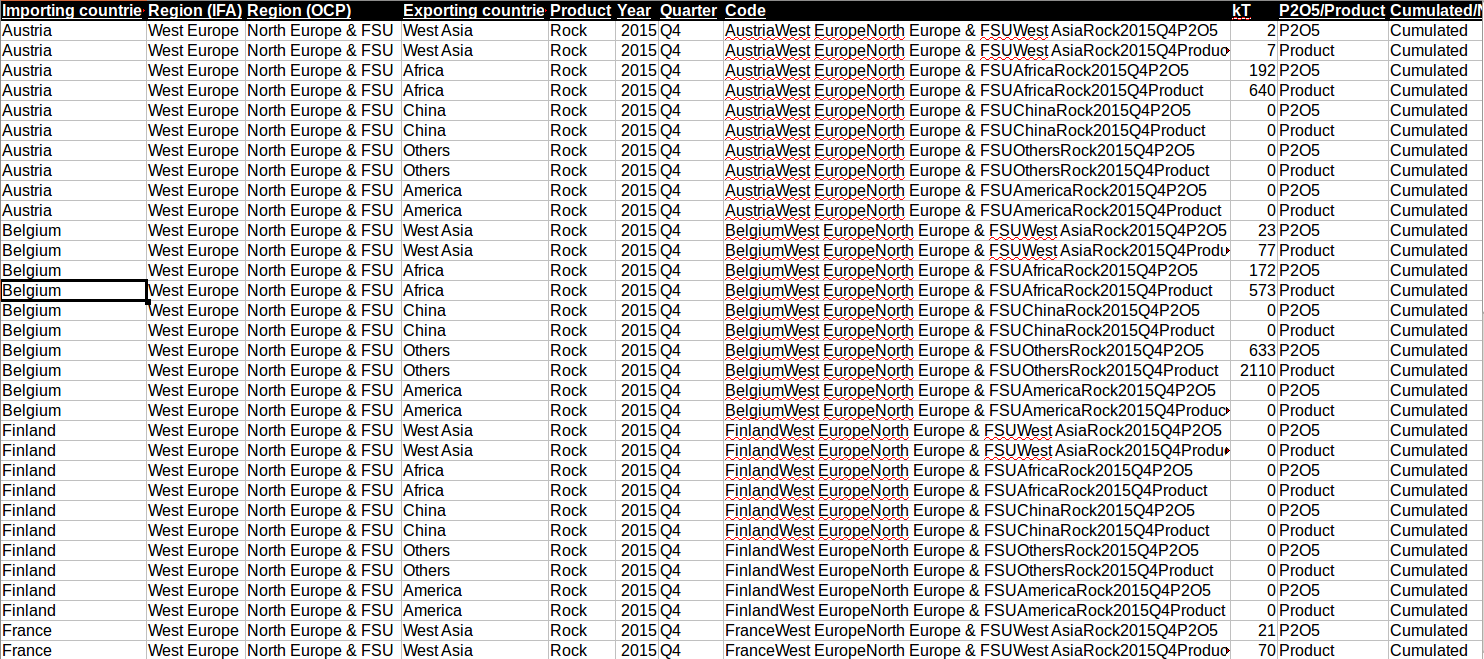
\includegraphics[scale=0.325]{Table}}
		    		\caption{Exemple d'une sortie de requête sur le Datamart OCP-CM}
		    		\label{fig:DMOCP}
	\end{figure}
	\subsection{Consolidation des données locales}
	Il est naturel d'adresser les problèmes de disponibilité de données aux premiers abords. La consolidation désigne la collection et l'intégration des données de sources multiples en une unique destination. Durant ce processus, nous unifierons les deux types de formats de données. Ceci nous permettra de présenter les données de manière plus flexible, tout en facilitant leur analyse effective. Ceci nous amène à considérer le format adopté par le datamart OCP-CM comme format cible de consolidation et les fichiers .pdf comme format source.
	\paragraph{}
	La solution que nous mettons en œuvre est disponible dans le dossier \textit{Sanxoriarty IFA Parser} du dépôt \textbf{GitHub} de notre mémoire de projet de fin d'études\cite{this}.
	\subsubsection{Conception fonctionelle}
	L'OCP reçoit régulièrement des rapports trimestriels présentant la situation du marché accompagnée des mouvements observés des produits fertilisants. Ces mouvements sont reportés sur des tableaux tel que celui présenté dans la figure \ref{fig:IFA-PDF}. Notre solution doit ainsi considérer les nuances fonctionnelles suivantes :\newpage
	\begin{enumerate}
	\item Les rapports diffèrent par leur granularité. En effet ceux-ci peuvent être:
		\begin{itemize}
		\item DET : Détaillés. Présentant l'historique des mouvements de produits entre les pays du monde deux-à deux.
		\begin{figure}[h]
					    		\centering
					    		\fbox{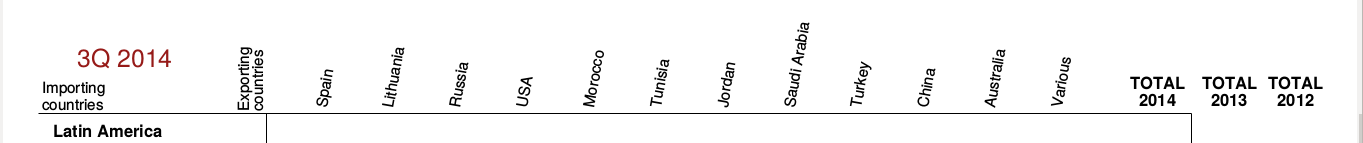
\includegraphics[scale=0.35]{det}}
					    		\caption{Exemple d'en-tête des tables du format DET des rapports IFA.}
				\end{figure}
		\item AGG : Agrégés. Présentant l'historique des mouvements entre les pays agrégés selon la région du monde à laquelle ceux-ci appartiennent.
		\begin{figure}[h]
			    		\centering
			    		\fbox{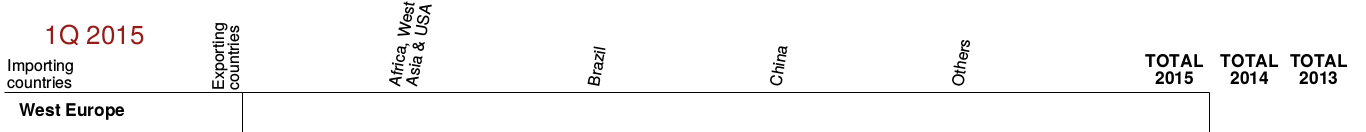
\includegraphics[scale=0.35]{agg}}
			    		\caption{Exemple d'en-tête des tables du format  AGG des rapports IFA.}
		\end{figure}
		\end{itemize}
	\item Les rapports diffèrent par les normes des chiffres rapportés. En effet ceux-ci peuvent être:
		\begin{itemize}
		\item NOT CUMULATED : Les chiffres rapportés au trimestre ${Q_i}$ sont bruts et représentent uniquement les ventes ayant effectivement eu lieu durant ce trimestre.
		\item CUMULATED : Les chiffres rapportés au trimestre ${Q_i}$ sont cumulés, i.e ${Q_i = \sum_{j=1}^{j=i} Q_j}$
		\item ANN : Les chiffres rapportés représentent toutes les ventes de l'année, i.e ${Q_i = \sum_{j=1}^{j=4} Q_j}$
		\end{itemize}
	\item Les attributs des enregistrements du datamart OCP-CM, sont des champs obligatoirement \textbf{NOT NULL} et sont les suivants:
	\begin{itemize}
	\item "Importing.countries" : Pays de destination de l'enregistrement-vente.
	\item "Region..IFA." : Région à laquelle appartient le pays de destination selon le découpage IFA.
	\item "Region..OCP." : Région à laquelle appartient le pays de destination selon le découpage OCP.
	\item "Exporting.countries" : Pays d'origine de l'enregistrement-vente.
	\item "Product" : Produit de l'enregistrement-vente. (MAP, DAP,PA\nomenclature{\textbf{PA : }}{Acide phosphorique},TSP ,ROCK\footnote{Minerai du phosphate brut en roche.})
	\item "Year" : Année de l'enregistrement-vente.
	\item "Quarter" Trimestre de l'enregistrement-vente.
	\item "Code" : Code de Synthèse des champs précédents.
	\item "kT" :  Poids de l'enregistrement-vente en kT\footnote{Kilotonne = $10^6$ kilogramme.} de produit.           
	\item "P2O5.Product" : Poids équivalent du produit en P2O5\footnote{Pentoxyde de phosphore, la molécule de base des engrais phosphatés.}
	\item "Cumulated.Not.cumulated" : Drapeau indiquant la norme trimestrielle de l'enregistrement-vente.
	\item "AGG.DET.ANN" : Drapeau indiquant la granularité de l'enregistrement-vente
	\end{itemize}
		Ainsi au-delà de la lecture des données contenues au sein des documents .pdf, ceux-ci doivent être:
		\begin{itemize}
		\item \textbf{Décumulés:} Des enregistrement des volumes unitaires par trimestre doivent être créés.
		\item \textbf{Convertis en P2O5:} Les données contenues dans les .pdf représentent les volumes échangés par kT qu'ils faut convertir selon la concentration du produit de l'enregistrement-vente en P2O5.
		\item \textbf{Normés:} La nature de l'agrégation trimestrielle de l'enregistrement-vente doit être spécifiée.
		\end{itemize}
	\end{enumerate}
	\subsubsection{Conception technique}\label{parser}
	\par
	La collecte et la préparation des données est un processus extrêmement lent et complexe,			\begin{wrapfigure}[14]{c}{8.4 cm}
						    		
						    		\fbox{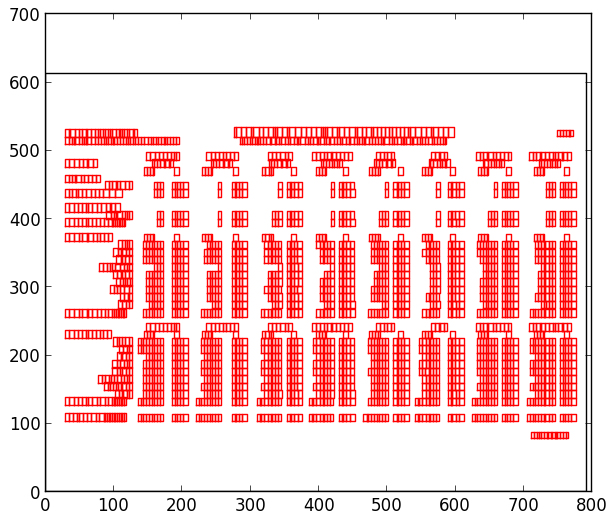
\includegraphics[scale=0.38]{charplot}}
						    		\caption{Représentation de l'information transportée par la page .pdf de la figure \ref{fig:IFA-PDF} pour une résolution d'image de 700x800.}
						    		\label{fig:charplot}
				\end{wrapfigure}  traditionnellement fait à la main et dont l'automatisation est souvent très difficile.
Le constat montre que 80 \% de la durée d'un projet Data Mining est consacrée à la récolte et la préparation des données\cite{DP}. Pour des données non structurées telles que des fichiers .pdf, la tâche est d'autant plus complexe. À la question : "Comment réaliser un \textit{Parsing} de fichiers PDFs", la réponse est souvent : "avec beaucoup de difficultés".

	\par
	PDF est un format de description de page et ne contient aucune information sur la structure logique d'un document telle que:\begin{itemize}
	\item L'emplacement du titre,
	\item Le début d'un paragraphe,
	\item Si la page est en une seule colonne ou plusieurs, etc.
	\end{itemize}
	\par
	Tout ce qu'un fichier .pdf indique est l'emplacement des caractères. La figure \ref{fig:charplot} ci-dessous montre comment les caractères sont disposés sur la page de la figure \ref{fig:IFA-PDF}.\\Une solution existe : \textbf{Tabula} de \textit{Mozilla} écrite en \textbf{Ruby} et précédemment utilisée par nos prédécesseurs (\cite{CHEMLAL},\cite{NACER}). Mais celle-ci présente l'inconvénient de nécessiter de l'utilisateur de dessiner des rectangles autour des tables cibles, ce qui n'offre aucun avantage d'automatisation.
	\par
	Notre solution utilise le package \textbf{pdfminer}\cite{pdfminer} du langage \textbf{Python} qui extrait les objets	\begin{wrapfigure}[16]{c}{8.4 cm}
			\centering			    		
			\fbox{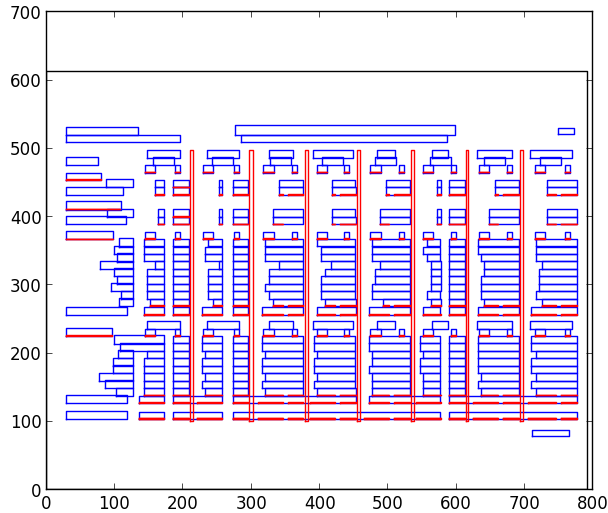
\includegraphics[scale=0.37]{classplot}}
			\caption{Classification de l'information transportée par la page .pdf de la figure \ref{fig:IFA-PDF}\\ selon ($\in$ zone de texte, $\notin$ zone de texte)}
			\label{fig:charclass}
		\end{wrapfigure}
		 non-texte et les mots de liaison en tant que blocs cohérents. Cette classification est montrée dans la figure \ref{fig:charclass} ci-contre. Les boîtes bleues indiquent où \textbf{pdfminer} a rassemblé un ensemble de caractères pour en faire des \textit{text boxes}\footnote{Zone de texte.} (cet ensemble de caractères peut être des mots ou des phrases) et les boites rouges indiquent les éléments non-texte (i.e, des lignes, des rectangles, etc.).
	\par
	La méthode utilisée par notre solution s'inspire des algorithmes d'analyse d'image et est similaire à la transformée de Hough utilisée par \textbf{Tabula}. Une transformée de Hough retrouve des segments de droites arbitrairement orientés dans une image. Notre problème, ici, est plus simple, nous nous intéressons uniquement au formes horizontales et verticales.
	\paragraph{}
	\begin{wrapfigure}[14]{c}{8.4 cm}
							\centering			    		
							\fbox{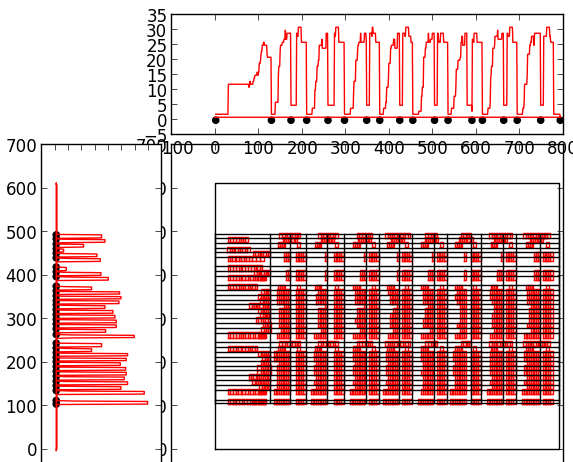
\includegraphics[scale=0.38]{projplot}}
							\caption{Inférence des frontières de la table de la figure \ref{fig:IFA-PDF}.}
							\label{fig:projplot}
						\end{wrapfigure}
	Pour trouver ces lignes verticales et ces colonnes, nous projetons les boites bleues (textuelles)sur l'axe horizontal (pour retrouver les colonnes\footnote{Nom du pays exportateur}) et sur l'axe vertical (pour retrouver les lignes\footnote{Données des enregistrements-ventes effectués par un pays importateur }). La projection consiste en l'énumération du nombre de boites bleues le long d'une ligne horizontale ou verticale. Nous concluons ainsi que les frontières entre les colonnes et les lignes sont marquées par les creux des valeurs des projections dans le graphe de projection; alors que les colonnes et les lignes en elles-même représentent les pics de la courbe. La figure \ref{fig:projplot} montre le résultat du traitement de la page de la figure \ref{fig:IFA-PDF}.\\Les graphes en haut et à gauche représentent le décompte des projections alors que les points noirs représentent les endroits où nous allons placer les frontières des lignes et des colonnes.
	\subsubsection{Conception du flux de données du processus de consolidation}
	La nature des transformations à faire subir les sources de données en vue de leur consolidation, nous amène à concevoir une solution technique en 2 phases:
	\begin{enumerate}
	\item \textbf{Une phase de structuration des données\footnote{cf. Annexe B1 pour le code-source}:}
	\begin{itemize}
	\item Nous parcourons l'arborescence contenant les .pdf source.
	\item Nous séparons le fichier .pdf en pages individuelles.
	\item Nous analysons les premiers caractères de la page en vue de labelliser chaque page selon si elle contient un produit, quel trimestre traite-elle, quelle normes les chiffres rapportés suivent-ils (cf. figure \ref{fig:IFA-TXT}).
	\item Nous faisons appel à notre outil de détection des tables discuté plus haut pour transformer chaque page-produit en une matrice de données.
	\item Nous compilons les matrices données d'un même produit en un seul fichier "data.csv" que nous confions au gestionnaire de fichier à placer dans une arborescence codifiant les données fonctionnelles de chaque fichier\footnote{cf. Annexe B3 pour plus de détails}.
	\end{itemize}
	\item \textbf{Une phase d'unification des modèles de données\footnote{cf. Annexe B2 pour le code-source}:}
	\begin{itemize}
	\item Nous parcourons l'arborescence générée par la phase précédente pour lire l'ensemble des "data.csv".
	\item Nous interrogeons le systèmes de fichier lors de la récupération de "data.csv" quant aux données fonctionnelles de celui-ci.
	\item Nous procédons si besoin aux opérations de décumulation et conversion.
	\item Les champs sont remplis conformément au modèle datamart OCP-CM (cf. figure \ref{fig:DMOCP}) et les données sont ainsi unifiées après audit de leur qualité.
	\end{itemize}
	\end{enumerate}
	Ces étapes sont résumées par le diagramme de flux de données de la figure \ref{fig:DF}.
		\begin{figure}[h]
		    		\centering
		    		\fbox{\includegraphics[scale=0.575]{dataflow}}
		    		\caption{Flux de données du processus de consolidation.}
		    		\label{fig:DF}
		\end{figure}
	\subsection{Audit et description des données locales consolidées}
	\subsubsection{Audit des données de consolidation}
	Lors de nos tests de la solution que nous avons mis au point lors de la section \ref{parser}, nous obtenions un taux de réussite de reconnaissance et extraction des tableau de 100\%. Cependant et de par la nature critique des données que nous traitons, nous avons procédé à tes tests rigoureux de deux natures différentes.
	\paragraph{Audit assisté par ordinateur:\\}
	Notre processus de consolidation a généré en moyenne près de 40800 enregistrements par année. Après une consolidation des années 2014, 2015 et début 2016, le total s'élève à 94240 nouveaux enregistrements dont nous nous devons d'assurer la justesse. Une vérification humaine un par un de chacun de ces enregistrements est une tâche pharamineuse que nous taclons en premier lieu en nous assistons du langage \textbf{R\footnote{\textbf{R} est un langage de programmation, de traitement des données et d'analyse statistique mettant en œuvre le langage de programmation \textbf{S}, avec la sémantique dérivée du langage \textbf{Scheme}}}.
\paragraph{}
		La figure \ref{fig:size} ci-dessous, valide bien le nombre d'enregistrements auxquels on s'attend, soit 94240 lignes. De plus, nous remarquons un premier soucis : Les cases de volumes nuls au sein de la colonne "kT" de la Trade Matrix ont été interprétés par le caractère "-". Ce qui empêche la colonne d'être traitée en tant que vecteur numérique. Nous remédions à ce problème en remplaçant ce caractère par le numérique "0", comme procédé dans la figure \ref{fig:nas} ci -après.
		\newline
			\begin{figure}[H]
			\begin{subfigure}{.5\textwidth}
				\centering
				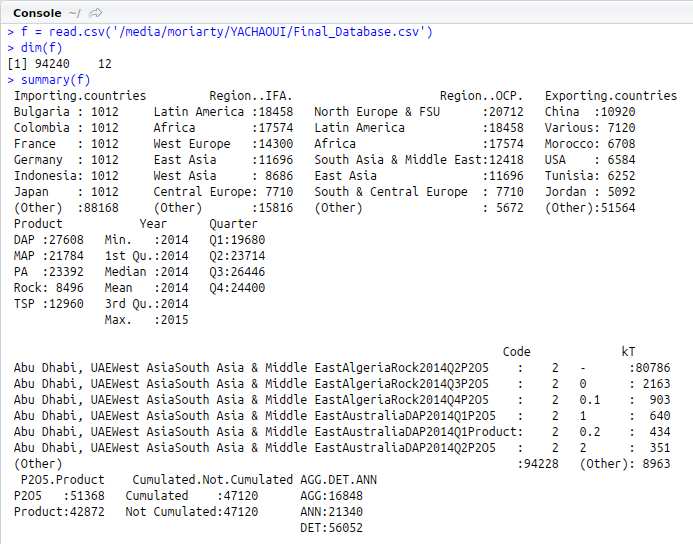
\includegraphics[height=215pt]{1}
				\caption{Vérification de la dimension\\des données consolidés}
				\label{fig:size}
			\end{subfigure}
			\begin{subfigure}{.5\textwidth}
					\centering
					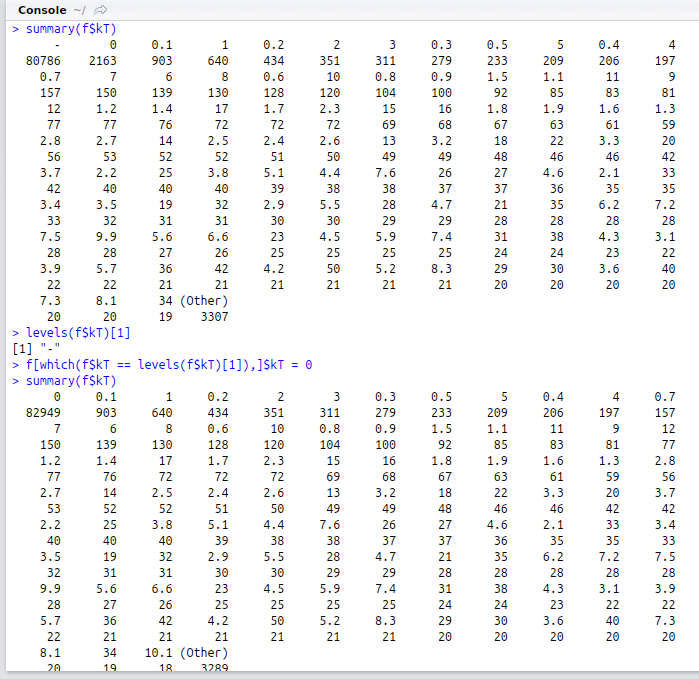
\includegraphics[height=215pt]{2}
					\caption{Traitement des cases vides\\des données consolidés}
					\label{fig:nas}
			\end{subfigure}
			\caption{Audit : Dimensions et données manquantes.}
				\end{figure}
				
	\paragraph{}
	Dans les figures \ref{fig:dubai} et \ref{fig:taiwan}, Nous observons deux interprétation différentes de \textbf{Dubai} en ("\textit{Dubai, UAE}","\textit{Dubai/ UAE}") et de \textbf{Taiwan} en ("\textit{Taiwan, China}","\textit{Taiwan/ China}"). Ces discrépances seraient analysées en tant que 4 pays différents alors qu'en réalité, ceux-ci ne sont que deux. Nous procédons à la correction de ces deux ambiguïtés dans les figures \ref{fig:corrDubai} et \ref{fig:corrTaiwan} respectivement.
	\begin{figure}[H]
	\begin{subfigure}{.5\textwidth}
			\centering
			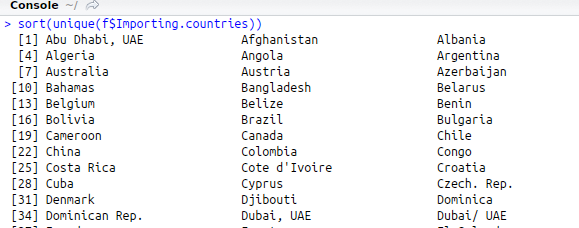
\includegraphics[height=90pt]{4}
			\caption{Ambiguïté Dubai, UAE}
			\label{fig:dubai}
	\end{subfigure}
	\begin{subfigure}{.5\textwidth}
		\centering
		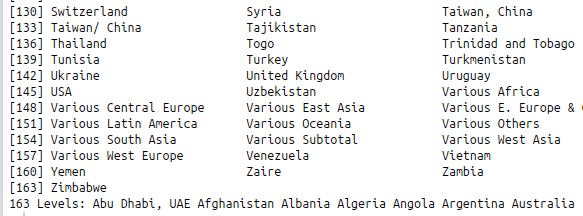
\includegraphics[height=90pt]{5}
		\caption{Ambiguïté Taiwan, China}
		\label{fig:taiwan}
	\end{subfigure}
	\begin{subfigure}{\linewidth}
			\centering
			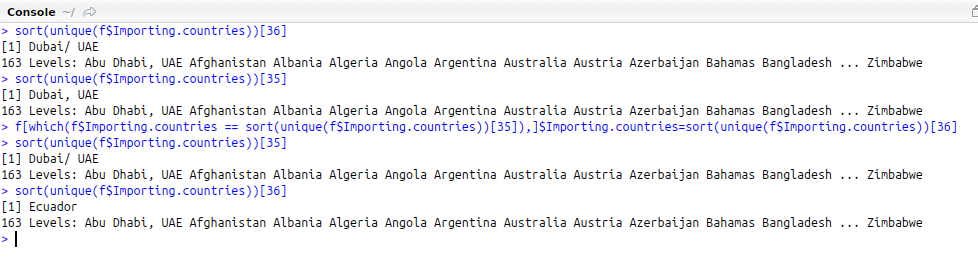
\includegraphics[width=\linewidth]{6}
			\caption{Correction Dubai, UAE}
			\label{fig:corrDubai}
	\end{subfigure}
	\begin{subfigure}{\linewidth}
			\centering
			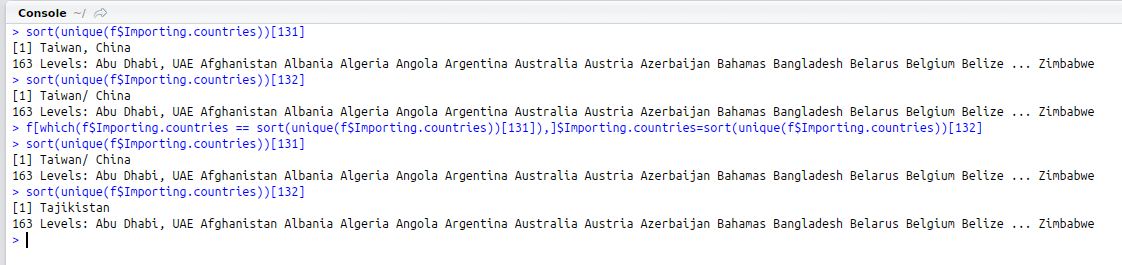
\includegraphics[width=\linewidth]{7}
			\caption{Correction Taiwan, China}
			\label{fig:corrTaiwan}
	\end{subfigure}
	\caption{Audit: Interprétation des chaînes de caractères.}
	\end{figure}
	\par
		
		\begin{figure}[H]
		\centering
		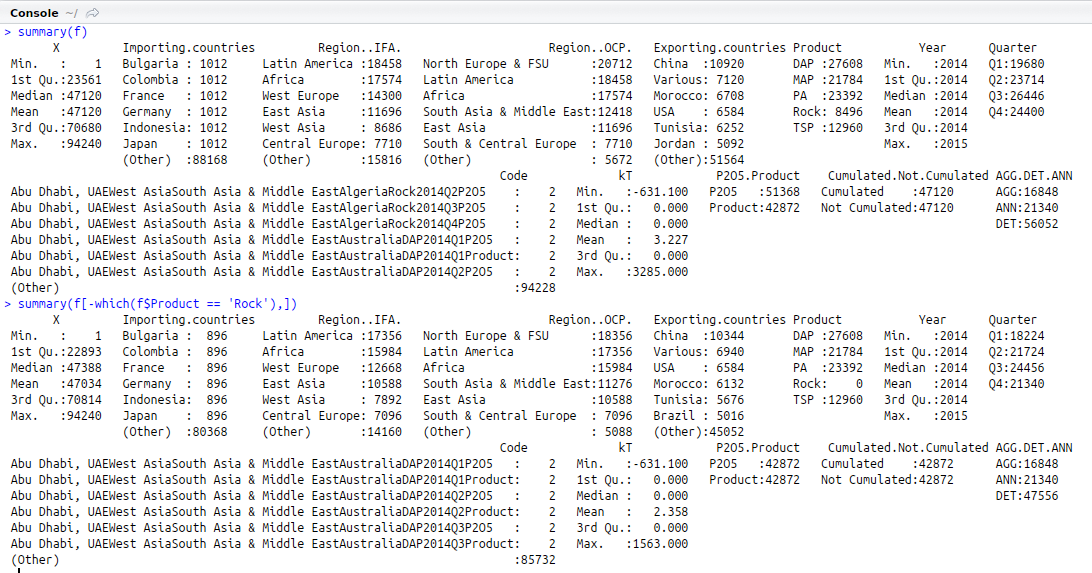
\includegraphics[scale=0.4]{8}
		\caption{}
		\label{fig:}
	\end{figure}
		\begin{figure}[H]
		\centering
		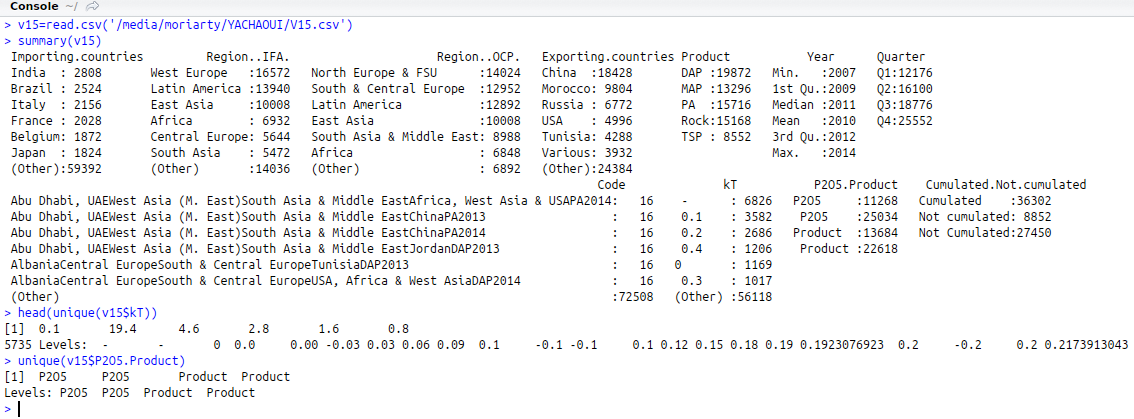
\includegraphics[scale=0.4]{9}
		\caption{}
		\label{fig:}
	\end{figure}
		\begin{figure}[H]
		\centering
		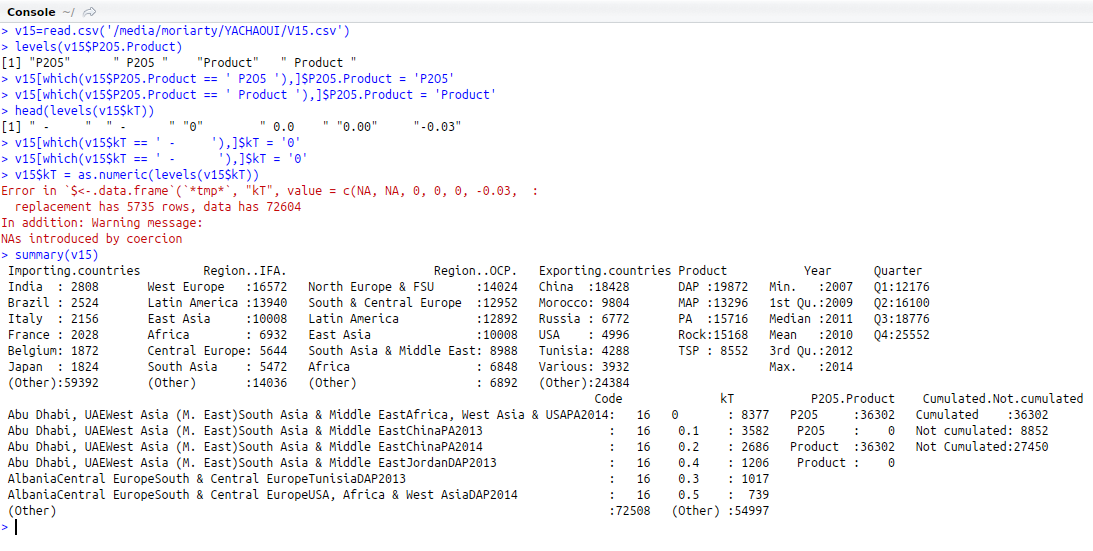
\includegraphics[scale=0.4]{10}
		\caption{}
		\label{fig:}
	\end{figure}
	\paragraph{Audit manuel d'échantillons aléatoires:}
	\subsubsection{Déscription des données de consolidation}
	\section{Collecte et préparation des données externes}
	L'étendue des données disponibles au sein du système d'information de l'OCP ne pouvant donner qu'une vue réduite de la situation du marché et ne peuvent de par leur définition révéler les structures socio-économiques,  et de politiques agraires sous-jacentes aux demandes en produits phosphatés, nous nous attellerons à la tâche d'enrichir cette base de données historiques par des données quantitatives concernant les pays du monde.
	\par
	Nous décrivons dans ce qui suit ce processus. 
	\subsection{Collecte des données externes}
	\subsubsection{Énumération et définitions des variables souhaitées }\label{exoList}
			Guidés par nos lectures bibliographiques résumées dans les sections \ref{read1} et \ref{read2}, nous nous fixons l'objectif de récolter les indicateurs de politiques agraires et socioéconomiques suivants:
	\begin{itemize}
		\item \textbf{ Access to electricity, rural (\% of rural population):} Fraction de paysans ayant accès à l'électricité.
		\item \textbf{ Access to non-solid fuel, rural (\% of rural population):} Fraction de paysans ayant accès aux fuels non solides.
		\item \textbf{ Account at a financial institution (\% age 15+):} Fraction de personnes âgées de +15 ans ayant un compte chez une institution bancaire.
		\item \textbf{ Net enrollment rate, primary (\% of primary school age children):} Fraction d'enfants scolarisés.
		\item \textbf{ Net national income per capita (constant 2005 US\$):} PIB\footnote{Produit intérieur brut, un des agrégats majeurs des comptes nationaux, il vise à quantifier — pour un pays et une année donnés — la valeur totale de la « production de richesse » effectuée par les agents économiques résidant à l’intérieur de ce territoire (ménages, entreprises, administrations publiques).} par habitant, inflation ajustée au dollar US fin 2005.\nomenclature{\textbf{PIB : }}{Produit intérieur brut}
		\item \textbf{ Literacy rate, adult total (\% of people ages 15 and above):} Fraction de personnes alphabétisées âgées de +15ans.
		\item \textbf{ Agricultural irrigated land (\% of total agricultural land):} Fraction de terres irriguées parmi les terres exploitées pour l'agriculture.
		\item \textbf{ Agricultural land (\% of land area):} Fraction des terres agricoles de la surface totale du pays.
		\item \textbf{ Agricultural tractors per 100 sq. km of arable land:} Nombre de tracteurs par 100 km² de terres arables.
		\item \textbf{ Agriculture, value added (\% of GDP):} Fraction de la valeur ajoutée agricole du PIB.
		\item \textbf{ Agriculture value added per worker (constant 2005 US\$):} Valeur ajoutée agricole par ouvrier agricol, inflation ajustée au dollar US fin 2005.
		\item \textbf{ All education staff compensation, total (\% of total expenditure in public institutions):} Fraction des dépenses en éducation des dépenses en institutions publiques.
		\item \textbf{ Annual freshwater withdrawals, agriculture (\% of total freshwater withdrawal):} Fraction du volume d'eau utilsée à des fins agricoles de la totalité de l'eau consommée.
		\item \textbf{ Arable land (\% of land area):} Fraction de terres arables de la surface totale du pays.
		\item \textbf{ Arable land (hectares per person):} Nombre d'hectares de terres arables par personne.
		\item \textbf{ Birth rate, crude (per 1,000 people):} Nombre de naissances par 1000 personnes.
		\item \textbf{ Cereal yield (kg per hectare):} Rendement des céréales en kilogramme par hectare.
		\item \textbf{ Commercial bank branches (per 100,000 adults):} Nombre d'agences bancaires par 100,000 adultes.
		\item \textbf{ Consumer price index (2010 = 100):} L'indice des prix à la consommation (IPC) mesure l'évolution du niveau moyen des prix des biens et services consommés par les ménages, pondérés par leur part dans la consommation moyenne des ménages. Harmonisé pour permettre une comparaison entre les pays à fin 2010.
		\item \textbf{ Cost to export (US\$ per container):} Coût en Dollars US de l'export d'un conteneur de marchandises.
		\item \textbf{ Cost to import (US\$ per container):} Coût en Dollars US de l'import d'un conteneur de marchandises.
		\item \textbf{ Crop production index (2004-2006 = 100):} 
		L'indice de production des cultures montre la production agricole pour chaque année par rapport à la période de base de 2004 à 2006. Cet indice porte sur l'ensemble des cultures à l'exception des cultures fourragères. Les regroupements par région et par revenu des indices de production de la FAO\nomenclature{\textbf{FAO : }}{Food and Agriculture Organization of the United Nations} sont calculés à partir des valeurs sous-jacentes en dollars US et normalisés par rapport à la période de référence de 2004 à 2006.
		\item \textbf{ Droughts, floods, extreme temperatures (\% of population, average 1990-2009):} Pourcentage moyen annuel entre 1990 et 2009 de la population affectée par les catastrophes naturelles classifiées comme sécheresses, inondations et évènements climatiques extrêmes.
		\item \textbf{ Employment in agriculture (\% of total employment):} Fraction des ouvriers agricoles de l'ensemble des employés.
		\item \textbf{ Food production index (2004-2006 = 100):} L'indice de production alimentaire porte sur les cultures vivrières qui sont considérées comme comestibles et qui contiennent des nutriments et normalisées par rapport à la période de référence de 2004 à 2006.
		\item \textbf{ GDP per capita (constant 2005 US\$):} PIB par habitant. Inflation ajustée à fin 2005.
		\item \textbf{ Household final consumption expenditure (constant 2005 US\$):}  La consommation privée désigne la valeur marchande de tous les biens et services, y compris les produits durables achetés par les ménages.
		\item \textbf{ Lending interest rate (\%):} Le taux d'intérêt perçu par les banques sur les prêts accordés aux clients.	
		\item \textbf{ Life expectancy at birth, total (years):} L'espérance de vie à la naissance indique le nombre d'années qu'un nouveau-né devrait vivre si les règles générales de mortalité au moment de sa naissance devaient rester les mêmes tout au long de sa vie.
		\item \textbf{ Livestock production index (2004-2006 = 100):} L'indice de production animale comprend la production de viande et de lait de toutes sources, les produits laitiers tels que le fromage, les œufs, le miel, la soie brute, la laine ainsi que les peaux et les cuirs.
		\item \textbf{ Logistics performance index:} La note globale de l'indice de performance de la logistique reflète les perceptions relatives à la logistique d'un pays basées sur l'efficacité des processus de dédouanement, la qualité des infrastructures commerciales et des infrastructures de transports connexes, la facilité de l'organisation des expéditions à des prix concurrentiels, la qualité des services d'infrastructure, la capacité de suivi et de traçabilité des consignations et la fréquence avec laquelle les expéditions arrivent au destinataire dans les délais prévus. L'indice varie continuellement de 1 à 5 et la note la plus élevée représente la meilleure performance.
		\item \textbf{ Low-birthweight babies (\% of births):} Fraction des nouveau-nés pesant moins de 2 500 grammes des naissances totales.
		\item \textbf{ Net migration:} Nombre d'immigrants total moins le nombre d'émigrants annuel, comprenant à la fois les citoyens et les non citoyens.
		\item \textbf{ Permanent cropland (\% of land area):} Fraction des terres occupées par des cultures pour de longues périodes et qui doivent être replantées après chaque récolte de la surface totale du pays.
		\item \textbf{ Population density (people per sq. km of land area):} Densité des habitants en personne par km².
		\item \textbf{ Population growth (annual \%):} Croissance relative annuelle de la population.
		\item \textbf{ Rural population (\% of total population):} Fraction rurale de la population.
		\item \textbf{ Rural poverty gap at national poverty lines (\%):} L'écart de pauvreté par rapport au seuil national de la pauvreté en milieu rural est le manque à gagner pour remonter au-dessus du seuil de la pauvreté (en considérant que les non pauvres ont un manque à gagner de zéro) exprimé en pourcentage du seuil national de la pauvreté en milieu urbain.Cette mesure témoigne à la fois de l'ampleur de la pauvreté et de sa fréquence.
		\item \textbf{ Unemployment, total (\% of total labor force):} Fraction de la population active qui est sans emploi mais qui est disponible pour et à la recherche d'un emploi.
		\end{itemize}
	\subsubsection{Recherche des sources WEB des variables souhaitées}
	\par
	\begin{Huge}{ Liste des cibles (sites web et bases de données publiques) du Crawling }
		\end{Huge}
	\subsubsection{Extraction et formatage des variables souhaitées}\label{crawl}
	\par
	 \begin{Huge}{ Workflow du  Crawling }
	 		\end{Huge}
	
	\subsection{Préparation des données externes}
	Cette section s’intéresse à l'application des forêts de décisions aléatoires à des fins de sélection de variables. Le but ici est double : d'abord introduire le comportement de l'indexation de l'importance des variables en utilisant les forêts aléatoires et l'utiliser pour proposer un algorithme à deux phases pour la sélection de variables à la base de leur importance.\par
	La stratégie générale se résume en un classement des variables exogènes\footnote{à savoir les variables externes "crawlées" dans la section \ref{crawl}.} en utilisant le score d'importance de ces variables introduit par les forêts aléatoires puis une sélection ascendante itérative des variables.
	\subsubsection{Introduction aux forêts de décision aléatoires}
	Les FA\nomenclature{\textbf{FA : }}{Forêts aléatoires} est un algorithme populaire et très efficient basé appartenant aux méthodes d'agrégation pour les problèmes de régression et de classification, introduit par Breiman\cite{BREI01}, et apparaît dans les application de 'Machine Learning'\footnote{L'apprentissage automatique ou apprentissage statistique (machine learning en anglais), champ d'étude de l'intelligence artificielle, concerne la conception, l'analyse, le développement et l'implémentation de méthodes permettant à une machine (au sens large) d'évoluer par un processus systématique, et ainsi de remplir des tâches difficiles ou impossibles à remplir par des moyens algorithmiques plus classiques.} à la fin du dernier millénaire\cite{DITRI99}. Les FA deviennent de plus en plus populaires et semblent être très robustes dans beaucoup d'applications bien qu'ils ne soient pas clairement théorisés mathématiquement\cite{BIA08}. Une introduction sommaire des FA est donnée en annexe A1.
	\par

	Le principe des FA est de combiner plusieurs arbres ($ê_i$) de décision CART\cite{BREI84} en utilisant plusieurs échantillons bootstrap de l'ensemble d'apprentissage \textbf{$L_n$} et de choisir aléatoirement à chaque nœud un sous-ensemble de \textit{k} variables exogènes $X_i$. 
	\par
	L'agrégation à laquelle procèdent les FA est d’autant plus performante que la corrélation entre les prédicteurs agrégés  (arbres CART\nomenclature{\textbf{CART : }}{Classification And Regression Trees}) est faible. Afin de diminuer cette corrélation, Breiman\cite{BREI01} propose de rajouter une couche d’aléa dans la construction des
	prédicteurs.  Nous attirons l'attention du lecteur vers l'annexe A2 pour une note sur CART et son utilisation au sein des FA. Sommairement, à chaque étape de CART, \textit{k} variables sont sélectionnées aléatoirement parmi les \textit{p} et la meilleure coupure est sélectionnée uniquement sur ces \textit{k} variables : \par
	\textbf{Algorithme Forêts aléatoires}
	\begin{itemize}
	\item[\textbf{Entrées:}]
	\item x, une nouvelle observation à prévoir.
	\item \textit{$L_n$}, l'échantillon.
	\item \textit{B}, le nombre d'arbres.
	\item \textit{k} $\in \mathbb{N}^* $, le nombre de variables candidates pour découper un nœud.
	\end{itemize}
	Pour i = 1,...,\textit{B}:
	\begin{itemize}
	\item Tirer un échantillon bootstrap dans \textit{$L_n$}.
	\item Construire un arbre CART sur cet échantillon bootstrap, chaque coupure est sélectionnée
	en minimisant la fonction de coût de CART sur un ensemble de \textit{k} variables choisies au
	hasard parmi les \textit{p}. On note $ê(.,\theta_i)$ l’arbre construit.
	\item[\textbf{Sortie:}]L’estimateur ${ê(x) =  \frac{1}{B} \sum_{i=1}^{B} ê_i(x,\theta_i)}$
	\end{itemize}	
	\subsubsection{Sélection des variables et élagage des données externes}
	Parmi les nombreuses sorties proposées par la fonction randomForest, deux se révèlent particulièrement intéressantes. \textbf{L'erreur Out-of-Bag} et \textbf{Le score FA d'importance des variables}. Nous définissons celles-ci rigoureusement dans l'annexe A3. Ces deux sorties nous permettent de proposer la procédure suivante à deux phases pour l'élimination itérative des variables les moins pertinentes:
	\paragraph{Phase 1. Élimination initiale et classement:}\begin{itemize}
	\item Nous modélisons par FA notre ensemble de données initial, comprenant la totalité des variables exogènes listées dans la section \ref{exoList}.
	\item Nous calculons les score FA d'importance des variables et nous éliminons les variables d'importance triviale.
	\item Nous classons les \textit{m} variables restantes par ordre descendant des score FA d'importance
	\end{itemize}
	\paragraph{Phase 2. Sélection des variables:}
	\begin{itemize}
	\item Nous construisons la collection itérative des modèles de FA employant les \textit{$\alpha$} premières variables selon leur classement de score d'Importance. Pour ${\alpha \in [1,\textit{m}]}$.
	\item Nous retenons les variables du modèle ayant réussi la plus faible erreur OOB.
	\end{itemize}
	

\chapter{Réalisation}

\cleardoublepage

	\section{Implementation de l'ETL}
	\section{Réalisation du noyau de prévisions}

\addcontentsline{toc}{chapter}{Conclusion}

\chapter*{Conclusion}


%\addcontentsline{toc}{chapter}{Bibliographie}

\chapter*{Bibliographie}

\footnotesize

\noindent $[1]$ \hspace{2pt} A. Plateaux et P. Lacharme, \textit{Organisation d’une architecture de santé respectueuse de la vie privée}, juin 2014.

%\noindent $[2]$ \hspace{2pt} J. Bossi, \textit{Technologies de l’information et de la communication et données de santé : pour un cadre juridique en phase avec les évolutions technologiques et les besoins du système de santé}, mai 2014, page 1.

\noindent $[2]$ \hspace{2pt} Adopté par l'Assemblée générale des Nations Unies. \textit{Guidelines for the regulation of computerized personal data files}, resolution 45/95, Décembre 1990.

\noindent $[3]$ \hspace{2pt} Commission européenne, \textit{Communication from the Commission to the european parliament, the council, the economic and social committee and the commitee of the regions}, 4 Novembre 2010.

\noindent $[4]$ \hspace{2pt} Union européenne, \textit{On the protection of individuals with regards to the processing of personal data and on the free movement of such data}, 1995.

\noindent $[5]$ \hspace{2pt} Union européenne, \textit{On the processing of personal data and the protection of privacy in the electronic communications sector}, 2002.

\noindent $[6]$ \hspace{2pt} \textit{European convention on human rights}, 1987.

\noindent $[7]$ \hspace{2pt} Gouvernement marocain, \textit{Bulletin Officiel n° 5714}, 5 mars 2009.

\noindent $[8]$ \hspace{2pt} S. Sadki et H. El Bakkali, \textit{PPAMH: A Novel Privacy-Preserving Approach for Mobile Healthcare}.


\subsubsection*{Webographie}

\footnotesize

\noindent $[W1]$ \hspace{2pt} Philippe Loizon, \textit{Le marché de la santé mobile explose}, 02 juillet 2013, [En ligne], Date de dernière mise à jour: 02 juillet 2013, Disponoble sur: \\
\scriptsize{\underline{http://lesclesdedemain.lemonde.fr/sante/le-marche-de-la-sante-mobile-explose\_a-11-2901.html}} \footnotesize, 25 juin 2015.

\vspace{8pt}
\paragraphmark

\noindent $[W2]$ \hspace{2pt} \textit{Le cadre juridique du partage d’informations dans les domaines sanitaire et médico-social: état des lieux et perspectives}, 22 août 2012, [En ligne], Disponoble sur: \\
\scriptsize{\underline{http://esante.gouv.fr/services/reperes-juridiques/le-cadre-juridique-du-partage-d-informations-dans-les-domaines-sanitaire}} \footnotesize, 27 juin 2015.

\vspace{8pt}
\paragraphmark

\noindent $[W3]$ \hspace{2pt} \textit{An Introduction to Agile Modeling}, [En ligne], Disponoble sur: \\
\scriptsize{\underline{http://www.agilemodeling.com/essays/introductionToAM.htm}} \footnotesize, 25 juin 2015.

\vspace{8pt}
\paragraphmark

\noindent $[W4]$ \hspace{2pt} \textit{Extreme programming}, [En ligne], Date de dernière mise à jour: 7 mars 2015, Disponoble sur: \\
\scriptsize{\underline{https://fr.wikipedia.org/wiki/Extreme\_programming}} \footnotesize, 25 juin 2015.

\vspace{8pt}
\paragraphmark

\noindent $[W5]$ \hspace{2pt} \textit{La e-santé de demain sera mobile},  21 septembre 2012, [En ligne], Disponoble sur: \\
\scriptsize{\underline{http://esante.gouv.fr/le-mag-numero-4/la-e-sante-de-demain-sera-mobile}} \footnotesize, 28 juin 2015.

\vspace{8pt}
\paragraphmark

\noindent $[W6]$ \hspace{2pt} \textit{Politique de confidentialité}, [En ligne], Date de dernière mise à jour: 19 mai 2012, Disponoble sur: \\
\scriptsize{\underline{https://fr.wiktionary.org/wiki/Wiktionnaire:Politique\_de\_confidentialité}} \footnotesize, 28 juin 2015.

\vspace{8pt}
\paragraphmark

\noindent $[W7]$ \hspace{2pt} \textit{Confidentialité}, [En ligne], Date de dernière mise à jour: 20 avril 2015, Disponoble sur: \\
\scriptsize{\underline{https://fr.wikipedia.org/wiki/Confidentialité}} \footnotesize, 28 juin 2015.

\vspace{8pt}
\paragraphmark

\noindent $[W8]$ \hspace{2pt} \textit{Politique de sécurité informatique}, [En ligne], Date de dernière mise à jour: 14 novembre 2014, Disponoble sur: 
\scriptsize{\underline{https://fr.wikipedia.org/wiki/Politique\_de\_sécurité\_informatique}} \footnotesize, 28 juin 2015.

\vspace{8pt}
\paragraphmark

\noindent $[W9]$ \hspace{2pt} \textit{Sécurité des applications mobiles : un enjeu difficile de l'ère BYOD mais pas une cause perdue},  06 février 2014, [En ligne], Disponoble sur: \\
\scriptsize{\underline{http://www.lemagit.fr/conseil/Securite-des-applications-mobiles-un-enjeu-difficile-de-lere-BYOD-mais-pas-une-cause-perdue}} \footnotesize, 28 juin 2015.

\vspace{8pt}
\paragraphmark

\noindent $[W10]$ \hspace{2pt} \textit{Auth0: Sequence Diagrams}, [En ligne], Disponoble sur:
\scriptsize{\underline{https://auth0.com/docs/sequence-diagrams}} \footnotesize, 28 juin 2015.


\vspace{8pt}
\paragraphmark

\noindent $[W11]$ \hspace{2pt} \textit{PhoneGap}, [En ligne], Disponoble sur:
\scriptsize{\underline{http://phonegap.com/}} \footnotesize, 28 juin 2015.

\vspace{8pt}
\paragraphmark

\noindent $[W12]$ \hspace{2pt} \textit{PhoneGap: Supported Features}, [En ligne], Disponoble sur: \\
\scriptsize{\underline{http://phonegap.com/about/feature/}} \footnotesize, 28 juin 2015.

\vspace{8pt}
\paragraphmark

\noindent $[W13]$ \hspace{2pt} \textit{10 frameworks JavaScript parmi les plus prometteurs}, 11 Octobre 2013, [En ligne], Disponoble sur: \\
\scriptsize{\underline{http://www.lemondeinformatique.fr/actualites/lire-10-frameworks-javascript-parmi-les-plus-prometteurs-55309.html}} \footnotesize, 28 juin 2015.

\vspace{8pt}
\paragraphmark

\noindent $[W14]$ \hspace{2pt} \textit{privacy policy}, [En ligne], Date de dernière mise à jour: 16 avril 2015, Disponoble sur: \\
\scriptsize{\underline{https://auth0.com/privacy}} \footnotesize, 28 juin 2015.

\addcontentsline{toc}{chapter}{Bibliographie}
\bibliographystyle{plain}
\bibliography{bibliographie}
%\addcontentsline{toc}{chapter}{Webographie}

\chapter*{Webographie}

\footnotesize

\noindent $[W1]$ \hspace{2pt} Philippe Loizon, \textit{Le marché de la santé mobile explose}, 02 juillet 2013, [En ligne], Date de dernière mise à jour: 02 juillet 2013, Disponoble sur: \\
\scriptsize{\underline{http://lesclesdedemain.lemonde.fr/sante/le-marche-de-la-sante-mobile-explose\_a-11-2901.html}} \footnotesize, 25 juin 2015.

\vspace{8pt}
\paragraphmark

\noindent $[W2]$ \hspace{2pt} \textit{Le cadre juridique du partage d’informations dans les domaines sanitaire et médico-social: état des lieux et perspectives}, 22 août 2012, [En ligne], Disponoble sur: \\
\scriptsize{\underline{http://esante.gouv.fr/services/reperes-juridiques/le-cadre-juridique-du-partage-d-informations-dans-les-domaines-sanitaire}} \footnotesize, 27 juin 2015.

\vspace{8pt}
\paragraphmark

\noindent $[W3]$ \hspace{2pt} \textit{An Introduction to Agile Modeling}, [En ligne], Disponoble sur: \\
\scriptsize{\underline{http://www.agilemodeling.com/essays/introductionToAM.htm}} \footnotesize, 25 juin 2015.

\vspace{8pt}
\paragraphmark

\noindent $[W4]$ \hspace{2pt} \textit{Extreme programming}, [En ligne], Date de dernière mise à jour: 7 mars 2015, Disponoble sur: \\
\scriptsize{\underline{https://fr.wikipedia.org/wiki/Extreme\_programming}} \footnotesize, 25 juin 2015.

\vspace{8pt}
\paragraphmark

\noindent $[W5]$ \hspace{2pt} \textit{La e-santé de demain sera mobile},  21 septembre 2012, [En ligne], Disponoble sur: \\
\scriptsize{\underline{http://esante.gouv.fr/le-mag-numero-4/la-e-sante-de-demain-sera-mobile}} \footnotesize, 28 juin 2015.

\vspace{8pt}
\paragraphmark

\noindent $[W6]$ \hspace{2pt} \textit{Politique de confidentialité}, [En ligne], Date de dernière mise à jour: 19 mai 2012, Disponoble sur: \\
\scriptsize{\underline{https://fr.wiktionary.org/wiki/Wiktionnaire:Politique\_de\_confidentialité}} \footnotesize, 28 juin 2015.

\vspace{8pt}
\paragraphmark

\noindent $[W7]$ \hspace{2pt} \textit{Confidentialité}, [En ligne], Date de dernière mise à jour: 20 avril 2015, Disponoble sur: \\
\scriptsize{\underline{https://fr.wikipedia.org/wiki/Confidentialité}} \footnotesize, 28 juin 2015.

\vspace{8pt}
\paragraphmark

\noindent $[W8]$ \hspace{2pt} \textit{Politique de sécurité informatique}, [En ligne], Date de dernière mise à jour: 14 novembre 2014, Disponoble sur: 
\scriptsize{\underline{https://fr.wikipedia.org/wiki/Politique\_de\_sécurité\_informatique}} \footnotesize, 28 juin 2015.

\vspace{8pt}
\paragraphmark

\noindent $[W9]$ \hspace{2pt} \textit{Sécurité des applications mobiles : un enjeu difficile de l'ère BYOD mais pas une cause perdue},  06 février 2014, [En ligne], Disponoble sur: \\
\scriptsize{\underline{http://www.lemagit.fr/conseil/Securite-des-applications-mobiles-un-enjeu-difficile-de-lere-BYOD-mais-pas-une-cause-perdue}} \footnotesize, 28 juin 2015.


\end{document}
